\section{Auswertung}
\label{sec:Auswertung}
%In dem Versuch sollte die spezifische molare Wärmekapazität einer Kupferprobe bestimmt werden. 
Die für die Molwärme charakteristische Materialgröße ist nach \eqref{eqn:cvd} die Debye-Temperatur $\theta_D$. 
Es wird beim Ohmmeter ein Messwiderstandsfehler von $\SI{0.1}{\ohm}$ erwartet.
\subsection{Messung der Molwärme}
Die Molwärme $C_V$ bei konstantem Volumen zu bestimmen, gestaltet sich experimentell schwierig. Leichter ist es, zunächst die Molwärme $C_P$ bei konstantem Druck zu bestimmen und diese mittels \eqref{eq:molwaermeconv}
umzurechnen. 
Die Molwärme $C_V$ kann mit der zugeführten Energie bestimmt werden. Diese kann aus den Werten in Tabelle \ref{tab:En} und Tabelle \ref{tab:tab1} mit
\begin{align}
	E &= U \cdot I \cdot \symup\Delta t,\\
	C_P &= \frac{M}{m}\cdot\frac{E}{\symup\Delta T}
	\label{eqn:cp}
\end{align}
berechnet werden. Dabei bezeichnen $M$ die molare Masse und $m$ die Probenmasse. Die Ergebnisse für die beiden Molwärmen sind dort auch eingetragen. 
Der lineare Ausdehnungskoeffizient $\alpha$ ist in Tabelle \ref{tab:al} eingetragen. Um diese genauer an die gemessenen Temperaturen anzupassen, wurden diese logarithmisch mit
\begin{equation*}
	\alpha_\text{fit}(x) = a\cdot\log{(b\cdot x + c)}
\end{equation*}
gefittet. Die Fitparameter sind dabei $a = \SI{-28 \pm 3}{}$, $b = \SI{
0.52\pm0.05}{}$ und $c = (\SI{3.47\pm0.07}{})\cdot 10^{-6}$.
Der Fit für $\alpha$ ist in Abbildung \ref{fig:a} zu sehen.
\begin{figure}
  \centering
  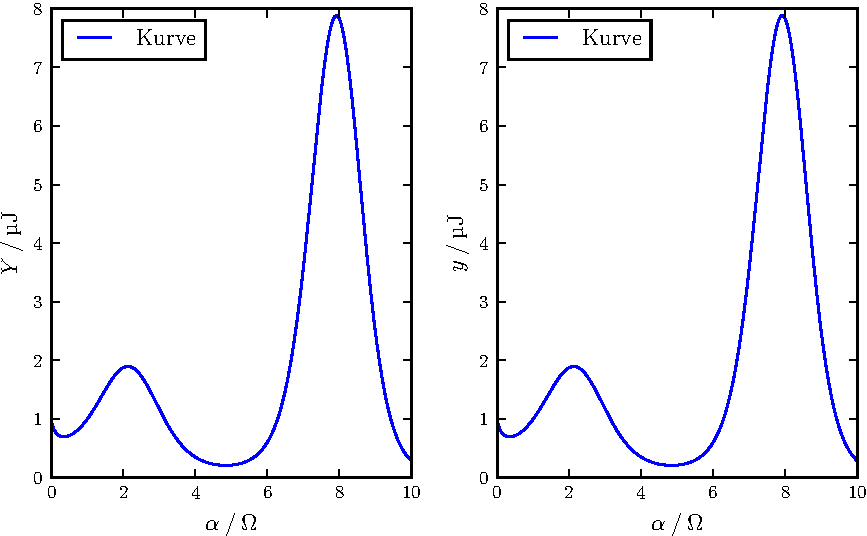
\includegraphics[width=\textwidth]{pc/plot.pdf}
  \caption{Der Fit für den linearen Ausdehnungskoeffizienten.}
  \label{fig:a}
\end{figure}
\begin{table}[h]
\centering
\caption{Die aufgenommene Wärmemenge berechnet mit den Messwerten für Strom und Spannung.}

\begin{tabular}{  S[round-mode=places, round-precision=1]  S[round-mode=places, round-precision=4]  S[round-mode=places, round-precision=2]  S[round-mode=places, round-precision=2] }
\toprule
{$U\:/\:\si\volt$} & {$I\:/\:\si\ampere$} & {$\Delta t \:/\:\si\second$} & {$E\:/\:\si\joule$} \\ \midrule
13.9&0.1335&322.23&597.9460995\\
18.8&0.1795&270.13&911.580698\\
19.9&0.1905&252.41&956.8736895\\
18.8&0.179&273.93&921.829236\\
18.85&0.1793&277.56&938.0986758\\
18.9&0.1795&282.9&959.752395\\
18.9&0.1795&297.49&1009.2496995\\
18.9&0.1797&319.18&1084.0406094\\
19.0&0.1798&322.8&1102.74936\\
19.0&0.1799&393.55&1345.193255\\
19.0&0.18&366.23&1252.5066\\
19.0&0.18&367.22&1255.8924\\
19.0&0.18&366.23&1252.5066\\
19.0&0.18&354.0&1210.68\\
19.0&0.18&378.0&1292.76\\
19.0&0.1802&398.7&1365.06906\\
19.0&0.1802&412.05&1410.77679\\
19.0&0.1802&382.84&1310.767592\\
19.0&0.1803&402.2&1377.81654\\
19.0&0.1803&401.55&1375.589835\\
19.0&0.1803&435.0&1490.1795\\
19.0&0.1804&407.04&1395.170304\\
19.0&0.1804&382.89&1312.393764\\
\bottomrule
\end{tabular}
\label{tab:LABEL}
\end{table}
\begin{table}[h]
\centering
\caption{Die Messwerte und die bereits berechneten Werte für die Wärmekapazitäten.}
\begin{tabular}{  S[round-mode=places, round-precision=1] S[round-mode=places, round-precision=1] @{${}\pm{}$}  S[round-mode=places, round-precision=1] S[round-mode=places, round-precision=1] @{${}\pm{}$}  S[round-mode=places, round-precision=1] S[round-mode=places, round-precision=1] @{${}\pm{}$}  S[round-mode=places, round-precision=1] S[round-mode=places, round-precision=1] @{${}\pm{}$}  S[round-mode=places, round-precision=1] }
\toprule
{$R\:/\:\si\ohm$} & \multicolumn{2}{c}{$T\:/\:\si\kelvin$} &\multicolumn{2}{c}{$\Delta T\:/\:\si\kelvin$} &\multicolumn{2}{c}{$C_P\:/\:\si{\joule\per\mole\per\kelvin}$} &\multicolumn{2}{c}{}{$C_V\:/\:\si{\joule\per\mole\per\kelvin}$} \\ \midrule
27.1&85.29786459999997&0.23595159999999998&x&x&x&x&x&x\\
31.3&93.33570939999996&0.23686279999999998&8.037844799999988&0.3343308893392891&13.742189549612418&0.5755524915717548&13.822434267464224&0.5749385384344802\\
35.5&103.30758459999998&0.2379884&9.971875200000028&0.33577144690756533&16.88196073249394&0.5725746411917922&16.985580680545354&0.5719358583300247\\
39.6&113.32673499999996&0.23911400000000002&10.019150399999972&0.3373632812422834&17.617637405144738&0.5981818589096461&17.74540148755374&0.5975204117908882\\
43.8&123.15293439999996&0.2402128&9.826199400000007&0.3389361212379702&17.279061379553614&0.6019545814797218&17.4311892170532&0.6012558285549484\\
47.9&133.26550959999997&0.24133839999999998&10.112575200000009&0.3405090492166104&17.058575857784458&0.5811398125731886&17.236491562726968&0.5803844458782647\\
52.0&143.18290939999997&0.24243720000000002&9.917399799999998&0.34208188969660464&17.777501730246744&0.6210183463600157&17.98139973095834&0.6202342673889428\\
56.1&153.14535999999998&0.24353599999999997&9.962450600000011&0.34363582356884737&18.592578627674367&0.6500935499175255&18.823247828313583&0.6492722051462969\\
60.0&163.15286139999998&0.2446348&10.007501399999995&0.34518975747701436&19.868921245346684&0.6950997203445519&20.127137082293306&0.6942473740891459\\
64.3&172.71399999999997&0.24568&9.561138599999992&0.3467057077278077&21.145227757157762&0.7779703587127615&21.43035241430348&0.7771067664114214\\
68.3&183.30301659999995&0.2468324&10.58901659999998&0.3482598111895198&23.28872710254765&0.7772408246437399&23.60430209653908&0.776316640338547\\
72.3&193.19775259999994&0.24790440000000002&9.894735999999995&0.3498325674220741&23.175410847293467&0.8325140409142814&23.520032853832593&0.831560688340527\\
76.3&203.13536859999994&0.2489764&9.937615999999991&0.35134860081736485&23.107501142012598&0.8312255110606114&23.48185130115716&0.8302107466481894\\
80.3&213.11586459999992&0.2500484&9.980495999999988&0.3528646342431046&22.9131843355053&0.8254984303579936&23.317930872373502&0.824415254370733\\
84.2&223.13924059999997&0.25112039999999997&10.023376000000042&0.35438066769890253&22.00702272770706&0.7946509343855452&22.442821660087287&0.7934753844362511\\
88.2&232.95331759999996&0.2521656&9.814076999999997&0.35587771090575476&24.00874710712257&0.8887048122163081&24.475442774700063&0.8875276348519636\\
92.1&243.06138159999995&0.2532376&10.108063999999985&0.3573748338609197&24.59376785376518&0.8884161863396833&25.092778476669753&0.8871656866447154\\
96.1&252.95802939999993&0.2542828&9.896647799999982&0.35887187745712257&25.95585298770123&0.9617391783256838&26.486971454112012&0.9604695818204629\\
100.0&263.1507813999999&0.2553548&10.192751999999984&0.36036900013580525&23.329755663390664&0.8462447475014027&23.89441212369996&0.8447969111630137\\
103.9&273.13&0.2564&9.979218600000081&0.36186604411444856&25.05617175441432&0.931718891009769&25.654111036308784&0.9302683955617328\\
107.8&283.14998139999994&0.2574452&10.01998139999995&0.36334417705949273&24.87666479943298&0.9265270808534414&25.508454996233958&0.9249866061294065\\
111.7&293.21072559999993&0.2584904&10.060744199999988&0.3648223100294169&26.855202335144682&0.9995371333824873&27.521404281404987&0.9979800783719026\\
115.5&303.3122325999999&0.2595356&10.10150699999997&0.3663004430239199&24.961580743154865&0.9322992547085023&25.662748454463358&0.9305815585814446\\
\bottomrule
\end{tabular}
\label{tab:LABEL}
\end{table}
\begin{table}[h]
\centering
\caption{Die angegebenen Werte für den linearen Ausdehnungskoeffizienten  \cite{skript}.}
\sisetup{%uncertainty-seperator = {\,},
table-number-alignment = center,
table-unit-alignment = center,
%table-figures-integer = 1,
%table-figures-decimal = 1,
table-auto-round = true
}
\begin{tabular}{S[table-format= 3.0] 
 S[table-format= 3.2] 
}
\toprule
{$T\:/\:\si\kelvin$}
&{$\alpha\:/\:\si{\per\micro\kelvin}$} \\
\midrule
70.0&7.0\\
80.0&8.5\\
90.0&9.75\\
100.0&10.7\\
110.0&11.5\\
120.0&12.1\\
130.0&12.65\\
140.0&13.15\\
150.0&13.6\\
160.0&13.9\\
170.0&14.25\\
180.0&14.5\\
190.0&14.75\\
200.0&14.95\\
210.0&15.2\\
220.0&15.4\\
230.0&15.6\\
240.0&15.75\\
250.0&15.9\\
260.0&16.1\\
270.0&16.25\\
280.0&16.35\\
290.0&16.5\\
300.0&16.65\\
\bottomrule
\end{tabular}
\label{tab:al}
\end{table}
\subsection{Bestimmung der Debye-Temperatur}
Um die Debye-Temperatur $\theta_D$ zu bestimmen, kann die Gleichung \eqref{eqn:cvd} genutzt werden. Das Integral ist tabellarisiert in Abbildung \ref{fig:cvd}
\begin{figure}
	\centering
	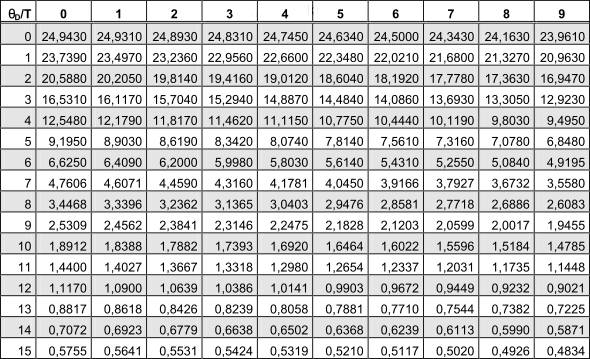
\includegraphics[width=0.8\textwidth]{graphics/cvd.png}
	\caption{Werte der Debye-Funktion.}
	\label{fig:cvd}
\end{figure}
zu sehen.
Die Werte können dann abgelesen und zur weiteren Berechnung genutzt werden.
Diese sind in Tabelle \ref{tab:deb} eingetragen.
\begin{table}[h]
\centering
\caption{CAPTION}
\sisetup{%uncertainty-seperator = {\,},
table-number-alignment = center,
table-unit-alignment = center,
%table-figures-integer = 1,
%table-figures-decimal = 1,
table-auto-round = true
}
\begin{tabular}{ S[table-format= 3.1]
 @{\,$\pm{}$\,} 
 S[table-format= 3.1] S[table-format= 3.1]
 @{\,$\pm{}$\,} 
 S[table-format= 3.1]  S[table-format= 3.1] 
S[table-format= 3.1]
 @{\,$\pm{}$\,} 
 S[table-format= 3.1] }
\toprule
\multicolumn{2}{c}{TITLE}
&\multicolumn{2}{c}{TITLE}
&{$\text{Title}$}
&\multicolumn{2}{c}{TITLE} \\
 \midrule
93.3357094&0.2368628&13.7421895495&0.575552491518&3.7&1.0&0.0\\
103.3075846&0.2379884&16.8819607323&0.572574641132&2.9&1.0&0.0\\
113.326735&0.239114&17.6176374049&0.598181858845&2.7&1.0&0.0\\
123.1529344&0.2402128&17.2790613793&0.601954581407&2.8&1.0&0.0\\
133.2655096&0.2413384&17.0585758576&0.581139812487&2.9&1.0&0.0\\
143.1829094&0.2424372&17.7775017301&0.621018346267&2.7&1.0&0.0\\
153.14536&0.243536&18.5925786275&0.650093549816&2.5&1.0&0.0\\
163.1528614&0.2446348&19.8689212452&0.695099720236&2.2&1.0&0.0\\
\bottomrule
\end{tabular}
\label{tab:LABEL}
\end{table}
Die Debye-Temperatur kann dann mittels \eqref{eqn:cvd} berechnet werden.
Es ergibt sich ein Mittelwert von
\begin{equation*}
	\theta_D = \SI{291\pm12}{\kelvin}
\end{equation*}
für die Debye-Temperatur.
Aus der Forderung \eqref{eqn:wd} kann die Debye-Temperatur für ein gegebenes Material auch bestimmt werden. Dazu muss die Verteilungsfunktion $Z(\omega)$ integriert und umgestellt werden.
Mit den Werten $m = \SI{342}{\gram}$, $v_\text{l} = \SI{4.7}{\kilo\metre\per\second}$ und $v_\text{tr} = \SI{2.26}{\kilo\meter\per\second}$ kann über
\begin{equation*}
	\theta_D = \frac{\hbar\omega_D}{k_\text{B}} = \SI{331.991}{\kelvin}
\end{equation*} bestimmt werden. 
